%%%%%%%%%%%%%% 
% Fichero: EjFigs
% Autor: J. Salido (http://www.esi.uclm.es/www/jsalido)
% Fecha: febrero, 2017
% Descripción: Ejemplo básico de inclusión de figuras.
% Ejemplo del curso: “LaTeX esencial para preparación de TFG, Tesis
% y otros documentos académicos” (Esc. Sup. Informática-UCLM)
%%%%%%%%%%%%%%




%%%%%%%%%%%%%%
% Preámbulo del documento
%%%%%%%%%%%%%%
\documentclass[11pt,a4paper]{article} 
\usepackage[spanish,es-tabla,es-noindentfirst]{babel} 
\usepackage[left=2cm,right=2cm,top=2cm,bottom=2cm]{geometry} % Márgenes 
\usepackage[skip=.3\baselineskip plus 2pt,indent]{parskip} % Salto entre párrafos 
% skip= .5\baselineskip plus 2pt -> Valor por defecto


% Tipografía
\usepackage{newtxtext}
\usepackage{newtxmath}

\usepackage{marvosym,pifont,textcomp,fontawesome5}

\usepackage[T1]{fontenc} % Codificación de salida    
\usepackage[
    protrusion=true,
    activate={true,nocompatibility},
    final,
    tracking=true,
    kerning=true,
    spacing=true,
    factor=1100]{microtype}
\SetTracking{encoding={*}, shape=sc}{40}


% Generación de hiperenlaces
\usepackage[%
   pdftex,
   breaklinks,
   hidelinks=true,      % Oculta colores en los enlaces (negro)
    linktocpage=true,    % true = enlace al nº de pág., false=texto completo
%    colorlinks=true,         % true=colorea texto del enlace, false=recuadra el texto
	citecolor=red, % Color de la citas
	urlcolor=blue, % Color de las URL
	bookmarksnumbered=true % Incluye números en bookmarks
]{hyperref}
\usepackage{url}
\urlstyle{sf} % Estilo de URL sin serifas


% Listas
\usepackage{enumitem} % Mayor control de listas
\usepackage{multicol} % Elementos en varias columnas

% Tablas
\usepackage{booktabs}

% Gráficos
\usepackage{graphicx}  % Inclusión de figuras y escalado de cajas
\usepackage{float} % Control de posición de objetos flotantes y estilos
\usepackage[margin=10pt,labelfont=bf]{caption}
\captionsetup[figure]{skip=5pt} % Necesario por si se desea colocar los títulos de las figs. en la parte superior. De este modo no queda tan pegado a la figura.

% Declaración del path donde están los archivos de figuras. 
% También se puede incluir el path en el nombre del fichero (tiene la ventaja de que TeXstudio muestra el fichero en tooltip)
\graphicspath{{../figs/}}  
\DeclareGraphicsExtensions{.pdf,.png,.jpg}
% Lista de extensiones de ficheros por orden de precedencia. De este modo no hace falta indicar la extensión del fichero y en caso de existir dos fichero con el mismos nombre y extensión diferente se emplea el que tiene una extensión con mayor prioridad.


% Con estas instrucciones se ajustan los valores del índice
\setcounter{secnumdepth}{2} % Ajusta el valor del último nivel numerado
\setcounter{tocdepth}{2} %Ajusta el valor del último nivel que aparece en TOC


\author{Jesús Salido}
\title{Inclusión básica de figuras en \LaTeX{}}
\date{\today}

%%%%%%%%%%%%%%
% Comienzo del documento
%%%%%%%%%%%%%%
\begin{document}

\maketitle

\begin{abstract}
	Explicación introductoria sobre cómo se incluyen y manejan las figuras con \LaTeX{}.
\end{abstract}

\hrule
\tableofcontents
\listoffigures
\bigskip
\hrule

\section{Primeros pasos}
La inclusión de figuras y archivos de imagen en un documento elaborado con \LaTeX{} es muy sencilla y versátil (en la Fig.~\ref{fig:plazaCR} se muestra una fotografía en formato \texttt{.jpg} en color).\footnote{El título de la imagen también muestra cómo debe darse créditos al autor de la imagen si esta no es de libre uso y tenemos permiso para usarla.} Hay que tener presente que el tipo de ficheros permitidos depende de si empleamos \texttt{latex} o \texttt{pdflatex},\footnote{En todo este curso asumimos que trabajaremos con \texttt{pdflatex} pues es más cómodo y siempre es posible utilizar la herramienta \texttt{epstopdf} para realizar la conversión de formatos.} ya que el primero sólo permite la inclusión de ficheros gráficos \texttt{.eps} mientras el segundo admite \texttt{.pdf}, \texttt{.png} y \texttt{.jpg}. Cuando la figura original presente un formato diferente a los mencionados, será preciso emplear algún programa para realizar la conversión apropiada. La inclusión de figuras requiere al menos el empleo del paquete \texttt{graphicx} con el que ya se pueden obtener resultados muy aceptables.

\begin{figure}[hbt] % Véase los tags de ubicación (h)ere, (b)ottom, (t)op 
	\centering % Fig. centrada en la página
% 	EDITAR: En caso de requerir que el título aparezca en la parte superior de la figura.
%	\caption[Ejemplo de foto en formato jpg]{La Plaza Mayor (cortesía de J.~Salido)} % Título y el título para la lista de figuras
%	\includegraphics[height=8cm]{plazaCR} % Alto de la figura en la pág.
	\includegraphics[height=8cm]{../figs/plazaCR} % Imagen en tooltip
	\caption[Ejemplo de foto en formato jpg]{La Plaza Mayor (cortesía de J.~Salido)} % Título y el título para la lista de figuras
	\label{fig:plazaCR} % Etiqueta para las refs. cruzadas
\end{figure}

\LaTeX{} puede procesar las figuras como \emph{objetos deslizantes o <<flotantes>>}\footnote{Estos elementos se denominan \textit{float} y por ello a veces en español utilizamos como traducción <<flotante>>.} (o sin ubicación prefijada). De este modo \LaTeX{} emplea algoritmos para encontrar la mejor ubicación de todos los objetos flotantes que contenga el texto. El usuario siempre tiene a su disposición opciones para sugerir la ubicación deseada dejando a \LaTeX{} la reubicación del texto y párrafos en la página. Con todo, en ocasiones el usuario debe hacer algunos ajustes para conseguir la ubicación deseada, aunque sigue siendo un procedimiento mucho más cómodo que en algunos de los procesadores de texto populares de tipo \textsc{wysiwyg}. Siempre que existan muchas figuras en el texto, el ajuste del resultado final va a ser más complejo y requerirá mayor intervención humana.

Otra de las ventajas de \LaTeX{} es que las imágenes no están incrustadas en nuestro fichero fuente, sino que son ficheros independientes incluidos durante la compilación. De este modo, la modificación de la figura no requiere cambios del fichero fuente sino únicamente una nueva compilación.








\section{Formatos gráficos}
A la hora de incluir figuras se debe decidir qué formato es el más apropiado siguiendo las siguientes reglas (resumidas de tabla~\ref{tab:formatos}):
\begin{itemize}
	\item Siempre que sea posible es preferible el formato \texttt{.pdf}, ya que es vectorial (escalable) como el gráfico de la Fig.~\ref{fig:4004arch}. Por supuesto, si el fichero \textsf{PDF} contiene alguna imagen de mapa de bits, esta no será escalable.
	\item Las fotografías se incluirán en formato \texttt{.jpg} (como en las  Figs.~ \ref{fig:plazaCR} y \ref{fig:mars}).
	\item Las capturas de pantalla o gráficos de gran contraste se deben incluir en formato \texttt{.png} (como en la Fig.~\ref{fig:inkscape}). 
	\item Siempre que se tenga un fichero de imagen (mapa de bits) con un fondo blanco u otro color plano, debería intentarse transformar en una imagen con fondo transparente convirtiéndola al formato \texttt{.png}.
\end{itemize}

\begin{figure}[hbt]
	\centering 
	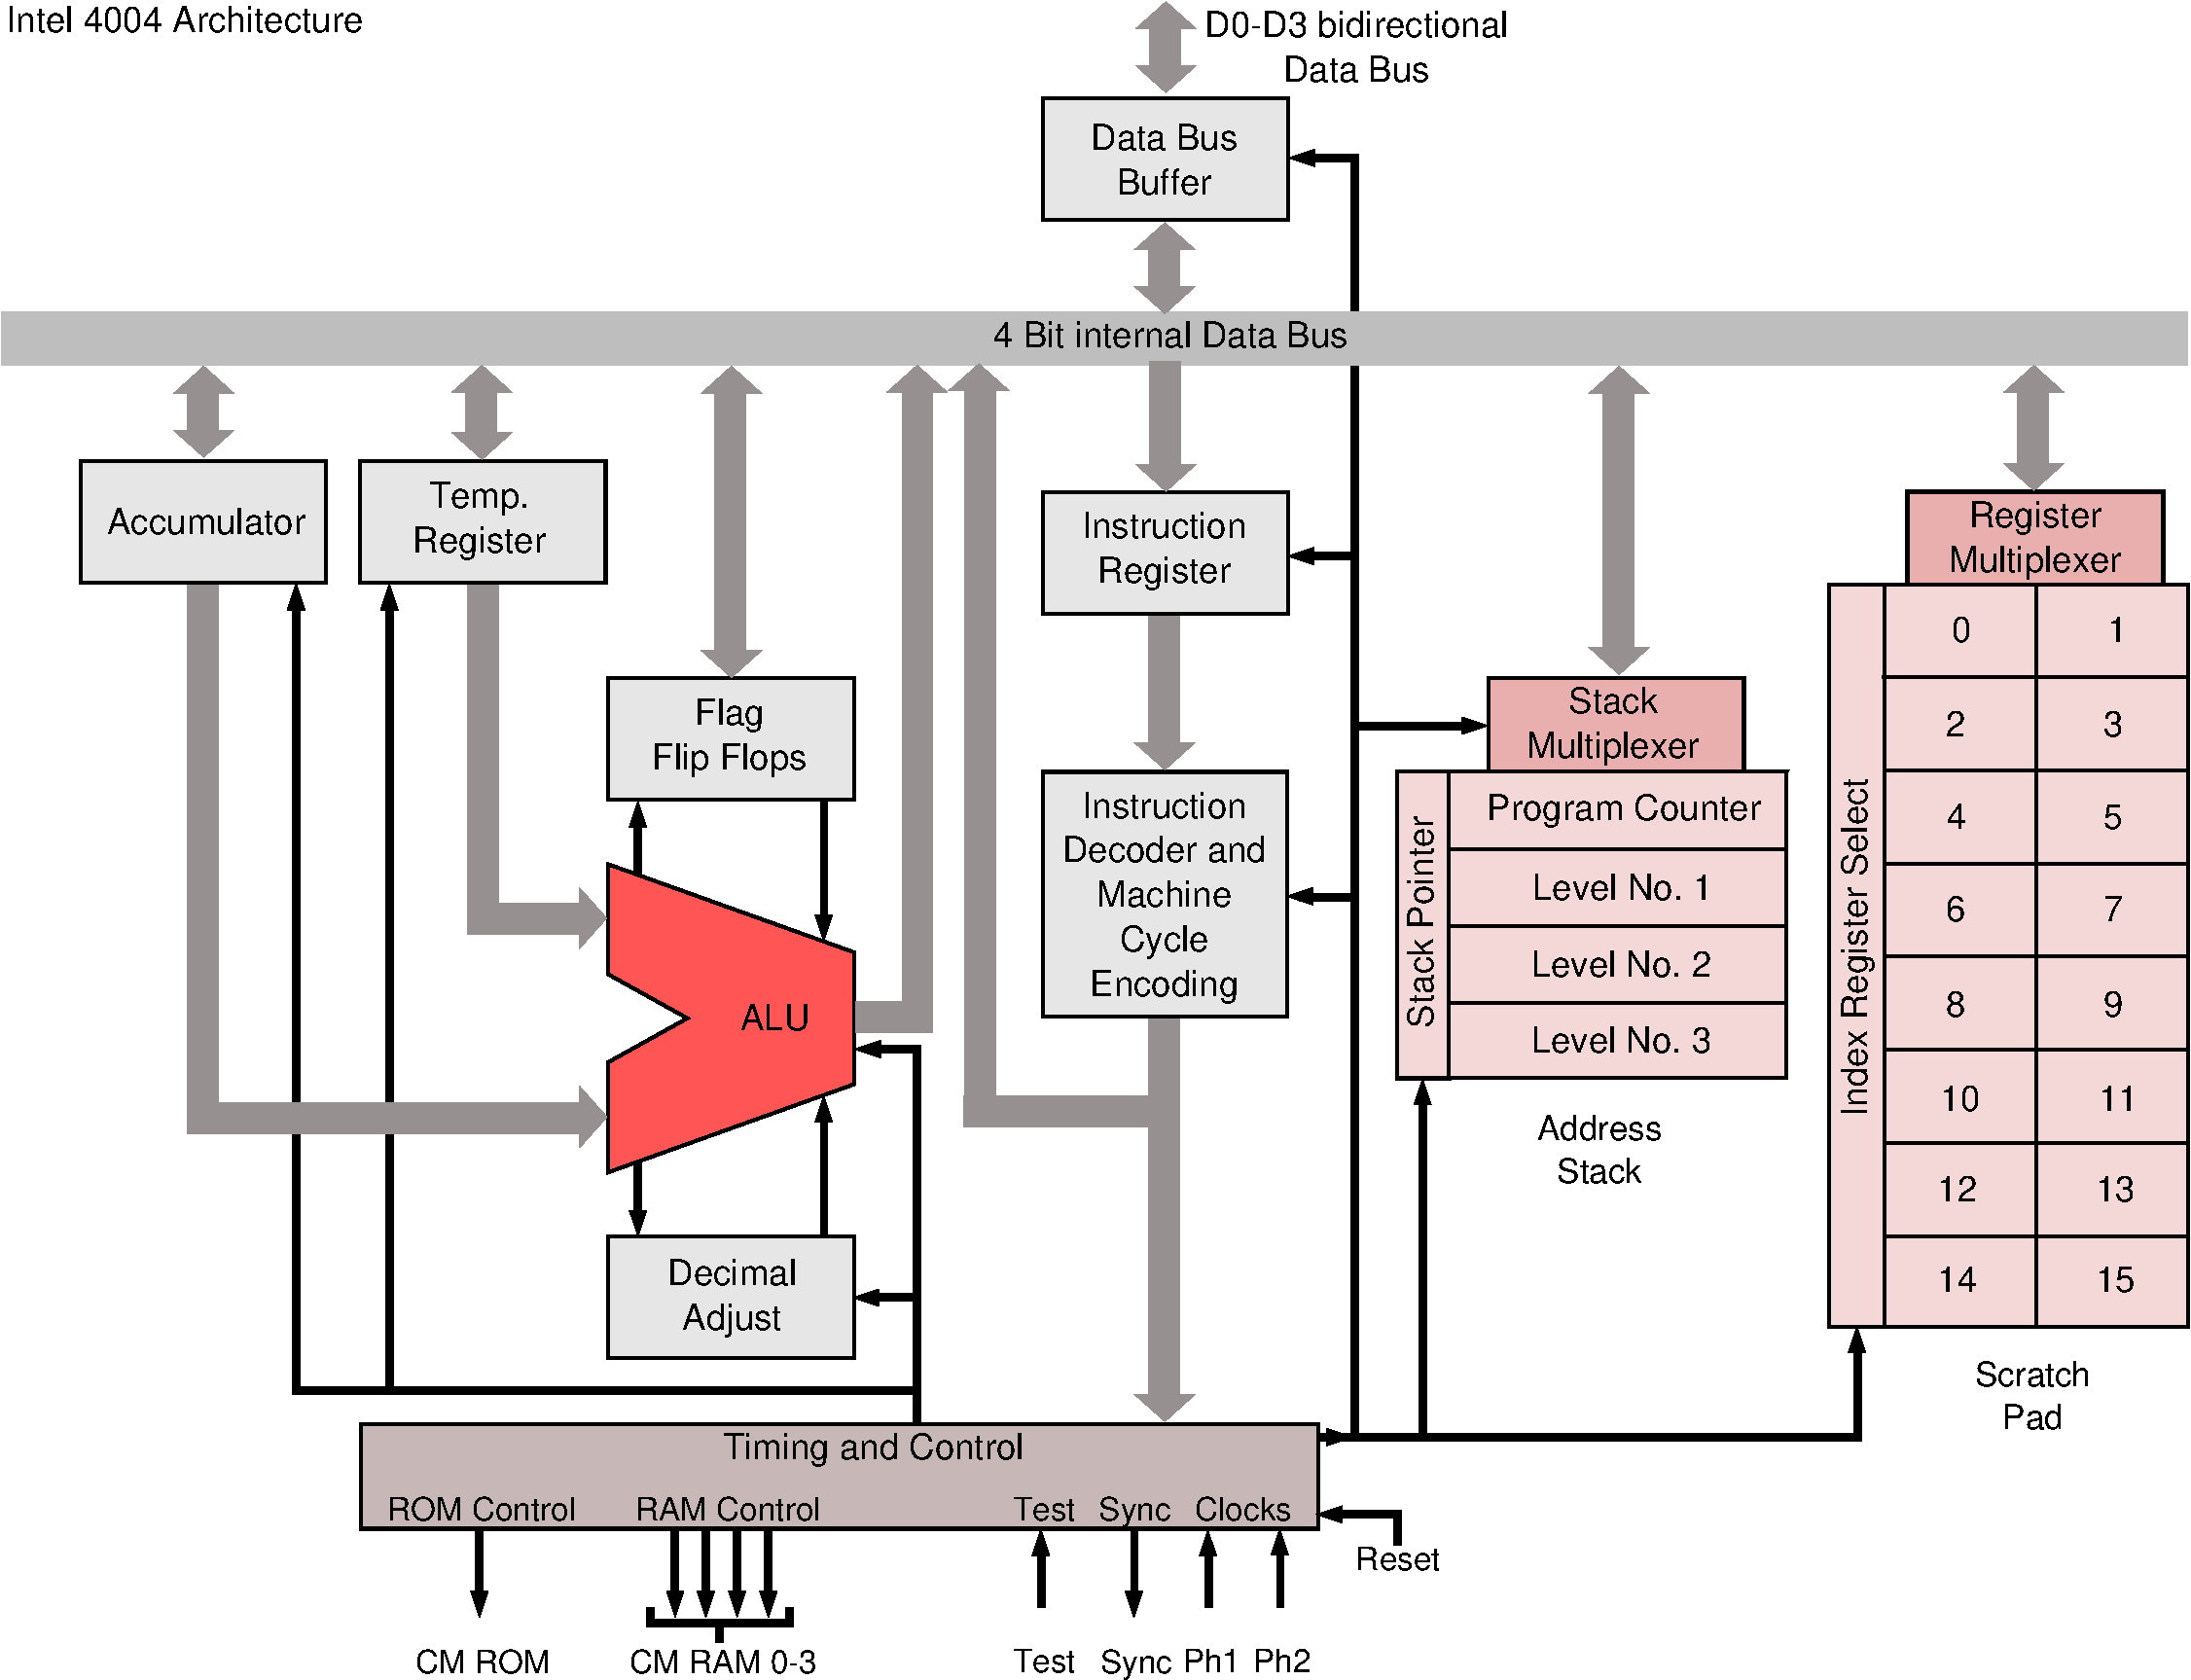
\includegraphics[width=0.65\textwidth]{../figs/4004arch} 
	\caption[Ejemplo de gráfico vectorial \textsf{PDF}]{Figura vectorial de arquitectura Intel 4004 en formato \textsf{PDF} (CC-BY-SA 3.0, Appaloosa, 2007. Wikimedia Commons)}
	\label{fig:4004arch}
\end{figure}

\begin{figure}[hbt]
	\centering
	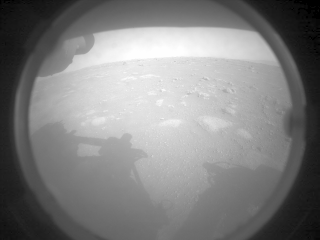
\includegraphics[width=0.6\textwidth]{Mars_Perseverance} 
	\caption[Foto histórica enviada desde Marte]{Primera foto enviada desde Marte el {18-2-2021} por el robot Perseverance incluida aquí en formato JPEG (cortesía de NASA/JPL-Caltech)}
	\label{fig:mars}
\end{figure}

\begin{figure}[hbt]
	\centering
	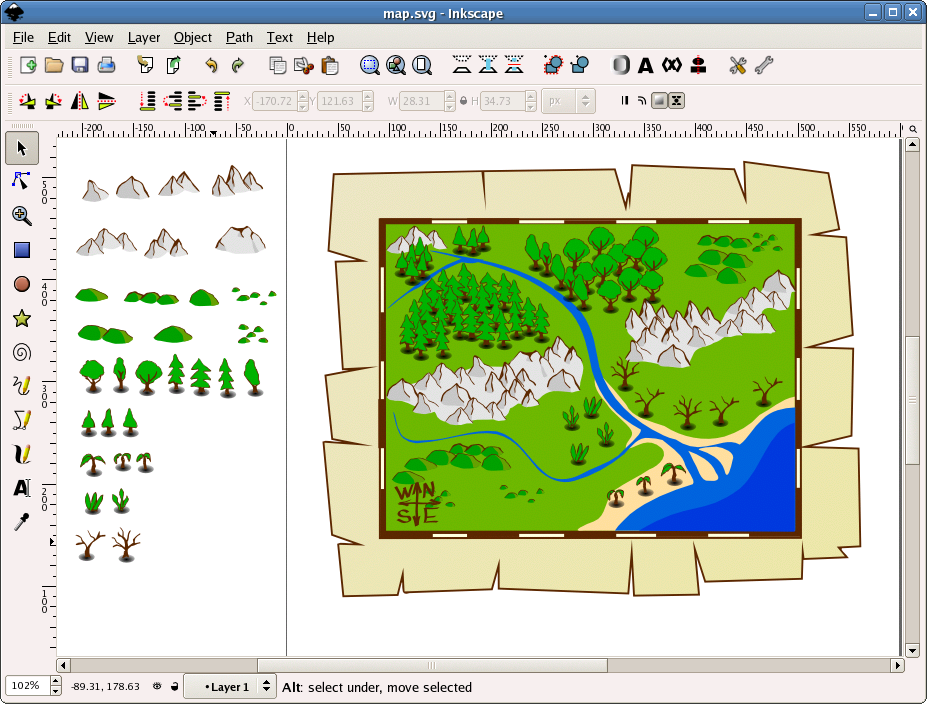
\includegraphics[width=0.5\textwidth]{../figs/inkscape} 
	\caption[Ejemplo de captura en png]{Captura de pantalla de \textsf{Inkscape} incluida en formato \textsf{PNG}}
	\label{fig:inkscape}
\end{figure}


\begin{table}[hbt]
\centering
\caption{Resumen de formatos de figuras y sus usos.}\label{tab:formatos}
\begin{tabular}{c|l}
\textbf{Formato} & \textbf{Uso} \\
\hline
PDF & Gráficos vectoriales \\
jpg & Imágenes (> 100 dpi) \\
png & Capturas de pantalla (> 75 dpi) 
\end{tabular}
\end{table}






\subsection{Ventajas del formato \textsf{PDF}}
Una de las dificultades de trabajar con ficheros \textsf{PDF} es que se trata de un formato difícil de editar, de modo que habitualmente se genera a partir de otros formatos. Por ejemplo, el gráfico de la Fig.~\ref{fig:4004arch}, cuyo formato original es \textsf{SVG}, ha sido realizado con el programa \textsf{Inkscape} y convertido al formato \textsf{PDF} mediante la herramienta de exportación que incluye (a través de \textsf{Cairo}). En los programas que no poseen una herramienta de exportación a formato \textsf{PDF}, este se puede generar imprimiendo a un archivo con un driver de impresión \textsf{PDF}. 

Cuando se trabaja con figuras hay que tener mucho cuidado con emplear imágenes de Internet sin tener la seguridad de los términos de uso de las mismas. Con mucha frecuencia al utilizarlos, se violan los derechos de propiedad intelectual, incluso cometiendo involuntariamente un delito. Por este motivo recomiendo recurrir a librerías de dominio público y licencias de libre uso como Creative Commons ---permiten el uso de las imágenes y \emph{cliparts} con pocas restricciones--- como por ejemplo OpenClipArt,\footnote{\url{http://openclipart.org/}} la página de galerías en el sitio de Inkscape\footnote{\url{http://wiki.inkscape.org/wiki/index.php/Galleries}} y Wikimedia Commons.\footnote{\url{http://commons.wikimedia.org/}} El derecho a cita permite la reproducción de figuras, sujetas a derechos restrictivos de distribución, en ámbitos académicos. Sin embargo, siempre debería incluirse en el pie de la figura la atribución de autoría y la licencia que se aplica a la distribución de la misma (no confundir con la licencia de nuestro documento). En cualquier caso debería investigarse la licencia de uso de la figura, puesto que en algunos casos (p.~ej.\ banco de imágenes de la \textsc{nasa}) el autor señala cómo debe realizarse la atribución de autoría. En ningún caso puede incluirse una figura ajena sin atribución, tanto si es de dominio público, como distribuida con una licencia permisiva.
\end{document}